\documentclass[10pt, fleqn]{beamer}
\usetheme{Montpellier}

\usepackage{xspace, alltt}
\usepackage[utf8x]{inputenc}

\usepackage{fontspec}
%\setmainfont{DejaVu Serif}

\setmonofont{DejaVu Sans Mono}[Scale=MatchLowercase]

\newcommand{\TODO}[2][]{[\textcolor{red}{TODO (#1):} \emph{#2}]}
\newcommand{\coq}{Coq\xspace}
\newcommand{\coqdoc}{Coqdoc\xspace}
\newcommand{\coqmakefile}{\texttt{coq\_makefile}\xspace}
\newcommand{\community}{Coq-community\xspace}
\newcommand{\gaia}{Gaia\xspace}
\newcommand{\alectr}{Alectryon\xspace}
\newcommand{\equations}{Equations\xspace}
\newcommand{\Hydras}{Hydras \& Co$\text.$\xspace}
\newcommand{\make}{\texttt{make}\xspace}

\definecolor{orange}{rgb}{1.0,0.6,0.0}
\definecolor{darkorange}{rgb}{0.7,0.25,0.0}
\definecolor{plugincolor}{rgb}{0.6,0.0,0.6}
\definecolor{mathcolor}{rgb}{0.0,0.0,0.6}
\definecolor{coqstylecolor}{rgb}{0.0,0.0,01.0}
\definecolor{lightblue}{rgb}{0.2,0.2,1.0}
\definecolor{metavarcolor}{rgb}{0.5,0.0,1.0}
\definecolor{darkgreen}{rgb}{0.1,0.7,0.1}
\definecolor{answercolor}{rgb}{.08,.15,.8}
\definecolor{normalcolor}{rgb}{0.0,0.0,0.0}
\definecolor{exbluecolor}{rgb}{0.1,0.1,0.9}
\definecolor{dontlookcolor}{rgb}{0.5,0.5,0.5}
\definecolor{termcolor}{rgb}{0.0,0.1,0.9}
\definecolor{lookcolor}{rgb}{0.5,0.1,0.0}
\definecolor{prooftermcolor}{rgb}{0.3,0.1,1.0}
\definecolor{typecolor}{rgb}{1.0,0.6,0.0}
\definecolor{taccolor}{rgb}{0.70,0.10,0.0}
\definecolor{pink}{rgb}{0.8,0.6,0.6}
\definecolor{darkmagenta}{rgb}{0.4,0.0,0.6}
\definecolor{darkblue}{rgb}{0.0,0.0,0.6}
\definecolor{cyan}{rgb}{0.0,0.4,0.8}
\usepackage{tikz}
\usepackage{tikzsymbols}
\usepackage{pifont}
\usetikzlibrary{arrows}

\usepackage{ifpdf}
\ifpdf
\usepackage{graphicx}
\else
\usepackage[dvips]{graphicx}
\fi

%%%% For Alectryon

\usepackage{texments}
\usepackage{./alectryon}
\usepackage{../pygments}

% Prevent breaks in the middle of syntactic units
\let\OldPY\PY
\def\PY#1#2{\OldPY{#1}{\mbox{#2}}}


%%% One hypothesis per line 
\makeatletter
\renewcommand{\alectryon@hyps@sep}{\alectryon@nl}
\makeatother

%%% \snippets{A,B,C,…} inputs a series of snippets as one block (with \itemsep
%%% between them).  A, B, C should be paths to files in snippets/.

\usepackage{etoolbox}
\makeatletter

\newcommand{\pathtomovies}{.}

\newcommand{\inputsnippets}[1]
{{\setlength{\itemsep}{1pt}\setlength{\parsep}{0pt}% Adjust spacing
    \alectryon@copymacros\begin{io}
      \forcsvlist{\item\@inputsnippet}{#1}
    \end{io}}}
\let\input@old\input % Save definition of \input
\newcommand{\@inputsnippet}[1]
{{\renewenvironment{alectryon}{}{}% Skip \begin{alectryon} included in snippet
    \input@old{{\pathtomovies}/#1}}}
\makeatother

% End of Alectryon stuff
%%%%%%%%%%%%%%%%%%%%%%%%%%%%%%%%%%%% 

%%%%%%% Specific macros

\newcommand{\canonseq}[2]{\mbox{$\{#1\}(#2)$}}
\newcommand{\rounds}{\mbox{\,\texttt{-+->}\,}}
\newcommand{\round}{\mbox{\,\texttt{-1->}\,}}
\newcommand{\rplus}[1]{\mbox{$\,\underset{#1}{\xrightarrow{\textcolor{white}{\,#1\,}}}\,$}}


\title{Hydras \& Co.: Formalized mathematics in Coq\\
  for inspiration and entertainment
}
\date{JFLA, June 2022}
\author{
  Pierre Castéran \inst{1}
  \and
  Jérémy Damour \inst{2}
  \and
  Karl Palmskog \inst{3}
  \and Clément Pit-Claudel \inst{4}
  \and Théo Zimmermann \inst{5}
}

\institute{
  Univ. Bordeaux, CNRS, Bordeaux INP, LaBRI, UMR 5800, F-33400 Talence, France  %\\
  % \email{pierre.casteran@labri.fr}
  \and
  Univ. de Paris, F-75013 Paris, France
  \and
  KTH Royal Institute of Technology, Stockholm, Sweden
  \and
  MIT CSAIL, Cambridge, Massachusetts, USA
  \and
  Inria, Univ. de Paris, CNRS, IRIF, UMR 8243, F-75013 Paris, France
}

%\usepackage[firstpage]{draftwatermark} 
\setbeamercolor{background canvas}{bg=}%transparent canvas

\begin{document}

%%%%%%%%%%%%%%%%%%%%%%%%%%%%%%%%%%%%

\begin{frame}
  \maketitle
\end{frame}

%%%%%%%%%%%%%%%%%%%%%%%%%%%%%%%%%%%%%% 
\begin{frame}
  \tableofcontents
\end{frame}
%%%%%%%%%%%%%%%%%%%%%%%%%%%%%%%%%%%%%%%
\section{Introduction}
%%%%%%%%%%%%%%%%%%%%%%%%%%%%%%%%%%%%%%%
\begin{frame}
    \frametitle{\community}
    \begin{block}{}
      \community is an informal organization that aims to maintain interesting open source \coq projects and facilitate collaboration among Coq users on documentation, tooling, etc.
      \begin{itemize}
      \item Created in 2018,  run by volunteer Coq users on GitHub
      \item At present, over than 50 projects, maintained by over than 30 volunteers
      \item Some packages were unmaintained before their integration to \community. According to their scientific or historical interest, we decided to revive them.
        \item After their transfer, packages may be the object of large changes  and refactorings.
      \end{itemize}
    \end{block}
  \end{frame}



%%%%%%%%%%%%%%%%%%%%%%%%%%%%%%%%%%%%%%%
\begin{frame}
  \frametitle{The \Hydras project}
  \begin{block}{}
    \begin{itemize}
   \item Experimental platform for the  development of \textcolor{lookcolor}{maintained} and \textcolor{lookcolor}{documented} libraries of formal proofs.
    \item A project of \community, developped on Github
      \begin{itemize}
      \item CI/CD
        \item Tools for collaboration (issues, PR, etc.)
        \end{itemize}
           \item A book in pdf (300p), generated  with \textcolor{lookcolor}{\alectr} and \LaTeX, continuously updated and deployed
    \end{itemize}
  \end{block}
  \begin{block}{Contents}
    \begin{itemize}
    \item Evolved version  of two contributions: \textcolor{plugincolor}{Cantor} and \textcolor{plugincolor}{Additions}
    \item Maintenance of \textcolor{plugincolor}{Ackermann}
      (part of Russel O'Connor's \textcolor{plugincolor}{Goedel})
    \item Bridge to \textcolor{plugincolor}{Gaia} (José Grimm) (\emph{in construction})
   
    \end{itemize}
  \end{block}
 
\end{frame}
%%%%%%%%%%%%%%%%%%%%%%%%%%%%%%%%%%%%%%%%%%%
\begin{frame}
  \frametitle{What hydras are talking about?}
  \begin{block}{}
    \Hydras presents a consistent set of examples, which allow us to formalize 
    some \textcolor{mathcolor}{discrete math}, discuss
    \textcolor{coqstylecolor}{\coq style, specification and proof patterns}, and depend on \textcolor{plugincolor}{a few plug-ins}.
  \end{block}
  \begin{block}{}
    \begin{description}
    \item[hydra battles:]
      
      \textcolor{mathcolor}{ordinals},
      \textcolor{mathcolor}{rapidly growing functions},
      \textcolor{mathcolor}{primitive recursive functions}, 
      \textcolor{coqstylecolor}{dependently typed functions},
      \textcolor{coqstylecolor}{operational type classes},
      \textcolor{coqstylecolor}{proofs of well-foundedness},
      \textcolor{coqstylecolor}{impossibility proofs},
      \textcolor{coqstylecolor}{uniqueness of identity proofs (UIP)},
      \textcolor{coqstylecolor}{indefinite description (Hilbert's epsilon operator)}, 
      \textcolor{plugincolor}{equations},
      \textcolor{plugincolor}{ackermann (goedel)},
      \textcolor{plugincolor}{gaia}
      
    \item[addition chains (exponentiation algorithms):]
      \textcolor{mathcolor}{algorithmics},
      \textcolor{mathcolor}{arithmetic},
      \textcolor{coqstylecolor}{operational type classes},
      \textcolor{coqstylecolor}{monadic notations},
      \textcolor{coqstylecolor}{PHOAS},
      \textcolor{coqstylecolor}{parametricity}, 
      \textcolor{plugincolor}{paramcoq}
    \end{description}
  \end{block}
\end{frame}

  %%%%%%%%%%%%%%%%%%%%%%%%%%%%%%%%%%%%%%%%%%%
\begin{frame}
  \frametitle{\Hydras: genealogy and dependencies}
\centering
\scalebox{0.6}{
\begin{tikzpicture}[thick]

  %%%%%%%%%%%% First line %%%%%%%%%%%%%%%%
  \begin{scope}[yshift=2.0cm, xshift=3cm]
     \node[ellipse, dotted, fill=orange!20, minimum height=0.5cm,minimum width=1.5cm] (algo) { Algorithmics};
     \node[ellipse, dotted, fill=orange!20, minimum height=0.5cm,minimum width=1.5cm, left of=algo, node distance=6cm] (settheory) { Set theory};
     \node[ellipse, dotted, fill=orange!20, minimum height=0.5cm,minimum width=1.5cm, left of=settheory, node distance=6cm] (prooftheory) {Proof theory};
  
\end{scope}

%%%%%% ACL2   %%%%%%%

\begin{scope}[yshift=1.0cm, xshift=-3.7cm]
   \node[rectangle, dotted, draw= black!20,fill=green!20,minimum height=0.5cm,minimum width=1.5cm] (acl2) { [ACL2]\footnote{P. Manolios \&  D. Vroon}};   
\end{scope}

%%%%%%% Contribs %%%%%%%%%%%%%%%%%%%%

\begin{scope}[xshift=-5.7cm]
\node[rectangle, dotted,draw=black,minimum height=0.5cm,minimum width=1.5cm] (goedel) { Goedel\footnote{R. O'Connor} };
\node[rectangle, dotted,draw=black,minimum height=0.5cm,minimum width=1.5cm,left of=goedel, node distance=2.2cm] (pock) { Pocklington\footnote{O. Caprotti \& M. Oostdijk}};
\node[rectangle, dotted,draw=black,minimum height=0.5cm,minimum width=1.5cm,right of=goedel, node distance=2.5cm] (cantor) { Cantor\footnote{C. \& E. Contejean}};

\node[rectangle, dotted,draw=black,minimum height=0.5cm,minimum width=1.5cm,right of=cantor, node distance=3.6cm] (cats) { Categories in ZFC\footnote{C. Simpson} };
\node[rectangle, dotted,draw=black,minimum height=0.5cm,minimum width=1.5cm,right of=cats, node distance=3.2cm] (additions) {Additions};

\end{scope}

%%%%%%%%%%%%%%%%% Plug-ins %%%%%%%%%%%%%%

\begin{scope}[yshift=-0.8cm,xshift=-1.2cm]
\node[rectangle, draw=black,minimum height=0.5cm,minimum width=1.5cm] (mathcomp) { MathComp };

  \node[rectangle, draw=black,fill=blue!30,minimum height=0.5cm,minimum width=1.5cm, right of=mathcomp, node distance=5.4cm] (paramcoq) { Paramcoq};

\node[rectangle, draw=black,minimum height=0.5cm,minimum width=1.5cm,node distance=2cm,left of=mathcomp, node distance=7.7cm] (equations) { Equations };
\end{scope}

\begin{scope}[yshift=-2cm,xshift=-4.2cm]
\node[rectangle, draw=black,fill=orange!80,minimum height=0.5cm,minimum width=1.5cm] (hydras) { Hydra-battles };
\node[rectangle, draw=black,fill=blue!30,minimum height=0.5cm,minimum width=1.5cm,left of=hydras, node distance=3.5cm] (pockcc) { Pocklington };
\node[rectangle, draw=black,fill=blue!30,minimum height=0.5cm,minimum width=1.5cm, right of=hydras, node distance=3.5cm] (gaia) { Gaia\footnote{J. Grimm} };


\node[rectangle, draw=black,fill=orange!80,minimum height=0.5cm,minimum width=1.5cm,right of=gaia, node distance=3.5cm] (chains) { Addition-chains };

\end{scope}

%%%%%%%%%%%%%%%%% goedel, etc . %%%%%%%%%%%%%%%
\begin{scope}[yshift=-3.7cm,xshift=-6cm]
 \node[rectangle, draw=black,fill=blue!30,minimum height=0.5cm,minimum width=1.5cm] (goedelcc) { Goedel };
 \node[rectangle, draw=black,fill=orange!80,minimum height=0.5cm,minimum width=1.5cm,right of=goedelcc, node distance=3cm] (gaiahydras) { Gaia-hydras };
\node[rectangle, draw=black,minimum height=0.5cm,minimum width=1.5cm,right of=gaiahydras, node distance=5.1cm] (alectryon) { Alectryon};
 
\end{scope}

\begin{scope}[yshift=-5cm,xshift=4cm]
\node[rectangle, draw=black,fill=red!80,minimum height=0.5cm,minimum width=1.5cm] (book) { \Hydras};  
\end{scope}

\draw[lookcolor,->,dotted] (acl2.south) -- (cantor.north) ;
\draw[lookcolor,->,dashed] (additions.south west) -- (chains.north) ;
\draw[lookcolor,->,dashed] (goedel) -- (goedelcc) ;
\draw[lookcolor,->,dashed] (goedel) -- (hydras.north) ;
\draw[lookcolor,->,dashed] (cantor) -- (hydras.north east) ;
\draw[lookcolor,->,dashed] (cantor.south) -- (gaia.north west) ;
\draw[lookcolor,->,dashed] (pock) -- (pockcc) ;
\draw[lookcolor,->,dashed] ([xshift=2.1cm]cats) -- (gaia) ;

\draw[->] (hydras.south) -- (gaiahydras) ;
\draw[->] (hydras.south west) -- (goedelcc) ;
\draw[->] (gaia.south west) -- (gaiahydras.north) ;

\draw[->] (equations) -- (hydras) ;
\draw[->] (mathcomp) -- (gaia) ;
\draw[->] (mathcomp) -- (chains) ;
\draw[->] (paramcoq.south) -- (chains) ;
\draw[->] (pockcc) -- (goedelcc) ;
\draw[dotted, ->] (prooftheory) -- (hydras);
\draw[dotted, ->] (settheory) -- (cats);
\draw[dotted, ->] (prooftheory) -- (goedel);
\draw[dotted, ->] (algo) -- (additions);
\draw[->, red] (alectryon) -- (book) ;
\draw[->, red] (chains) -- (book) ;
\draw[->, red] (gaiahydras) -- (book) ;
\draw[->, red] (hydras.south) -- (book) ;

\end{tikzpicture}
}
% \caption{Genealogy and dependencies for \Hydras.}
%   \label{fig:genealogy}
% \end{figure}
\end{frame}


%%%%%%%%%%%%%%%%%%%%%%%%%%%%%%%%%%%%%%%






% \begin{frame}
%   \frametitle{Yet another book on \coq?}
%   \begin{table}
%   \centering
%   \footnotesize
%   \begin{tabular}{lll}
%   \hline
%   \textbf{Title} & \textbf{Year} & \textbf{Category}\\
%     \hline
%    \coq reference manual &  $\geq 1989$ & \\
%   Coq'Art & 2004 & Traditional\\
%   Software Foundations & 2007 & Executable\\
%   Certified Programming with Dependent Types & 2011 &  Executable\\
%   Program Logics for Certified Compilers & 2014 & Traditional\\
%   Programs and Proofs & 2014 & Executable\\
%   Formal Reasoning About Programs& 2017 & Traditional\\
%   Computer Arithmetic and Formal Proofs & 2017 & Traditional\\
%     Mathematical Components & 2018 & Traditional\\
%   \hline
%   \end{tabular}
%   \caption{Coq book categorization.}
%   \label{tbl:books}
% \end{table}
  
% \end{frame}

%%%%%%%%%%%%%%%%%%%%%%%%%%%%%%%%%%%%%%%%%

% \begin{frame}
%    \begin{block}{An example-driven book}
%     \begin{itemize}
%     \item The structure is determined by the presented topics (discrete math, algorithmics, etc.). \coq technology (formalization and proof patterns) is presented when needed.
%     \item No need to be complete (there is already a reference manual)
%  %   \item No need to introduce \coq (there are already a lot of initiation books and tutorials)
%     \item Comparison of  different formalizations of a given notion, and several proofs of the same theorem.
%       \item Show also interesting dead ends (formalization, tactics, proof structure).
%     \end{itemize}
%   \end{block}
%   % \begin{block}{Examples}
%   %   \begin{itemize}
%   %   \item Tsukuba Coq Users's Group: regular languages, $\lambda$-calculus, arithmetic, ... (in Japanese + ssreflect)
%   %   \item Software Foundations (B. Pierce \emph{et al.})
%   %   \end{itemize}
%   % \end{block}
% \end{frame}

%%%%%%%%%%%%%%%%%%%%%%%%%%%%%%%%%%%%%%%%%%%% 


%%%%%%%%%%%%%%%%%%%%%%%%%%%%%%%%%%%%%%%

\section{Kirby \& Paris' hydras}

\begin{frame}
  \frametitle{Kirby \& Paris' hydras}
  \begin{figure}[h]
    \centering
    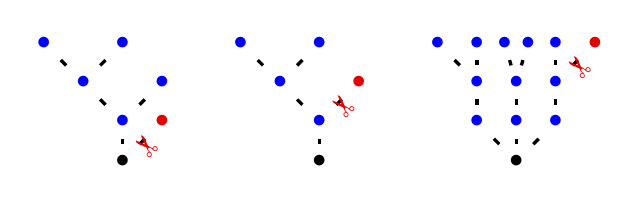
\begin{tikzpicture}[very thick, scale=0.25]
      \node (h1) at (4,0){$\bullet$};
      \node[blue] (h2) at (4,2){$\bullet$};
      \node[blue] (h3) at (2,4){$\bullet$};
      \node[blue] (h4) at (0,6){$\bullet$};
      \node[red!90!black] (h7) at (6,2){$\bullet$};
      \node[blue] (h5) at (4,6){$\bullet$};
      \node[blue] (h6) at (6,4){$\bullet$};
      \draw (h1) -- (h2) ;
      \draw (h2) -- (h3) ;
      \draw (h1) -- node[red!90!black,font=\small,sloped,
      shift={(0.01,-0.075)},rotate=90]{\textbf{\ding{34}}} (h7);
      \draw (h3) -- (h4) ;
      \draw (h3) -- (h5) ;
      \draw (h2) -- (h6);

      \node (h11) at (14,0){$\bullet$};
      \node[blue] (h12) at (14,2){$\bullet$};
      \node[blue] (h13) at (12,4){$\bullet$};
      \node[blue] (h14) at (10,6){$\bullet$};
      \node[blue] (h15) at (14,6){$\bullet$};
      \node[red!90!black] (h16) at (16,4){$\bullet$};
      \draw (h11) -- (h12) ;
      \draw (h12) -- (h13) ;
      \draw (h12) -- node[red!90!black,
      font=\small,sloped,shift={(0.01,-0.075)},
      rotate=90]{\textbf{\ding{34}}} (h16);
      \draw (h13) -- (h14) ;
      \draw (h13) -- (h15) ;
      
      \node (hn1) at (24,0){$\bullet$};
      \node[blue] (hn2) at (22,2) {$\bullet$};
      \node[blue] (hn3) at (22,4) {$\bullet$};
      \node[blue] (hn4) at (20,6){$\bullet$};
      \node[blue] (hn5) at (22,6){$\bullet$};
      \draw (hn1) -- (hn2) ;
      \draw (hn2) -- (hn3) ;
      \draw (hn3) -- (hn4) ;
      \draw (hn3) -- (hn5) ;
      \node [blue](hn2b) at (24,2) {$\bullet$};
      \node[blue] (hn3b) at (24,4) {$\bullet$};
      \node [blue](hn4b) at (23.4,6){$\bullet$};
      \node [blue](hn5b) at (24.6,6){$\bullet$};
      \draw (hn1) -- (hn2b) ;
      \draw (hn2b) -- (hn3b) ;
      \draw (hn3b) -- (hn4b) ;
      \draw (hn3b) -- (hn5b) ;
      \node [blue](hn2c) at (26,2) {$\bullet$};
      \node [blue](hn3c) at (26,4) {$\bullet$};
      \node [blue](hn4c) at (26,6){$\bullet$};
      \node [red!90!black] (hn5c) at (28,6){$\bullet$};
      \draw (hn1) -- (hn2c) ;
      \draw (hn2c) -- (hn3c) ;
      \draw (hn3c) -- (hn4c) ;
      \draw (hn3c) -- node[red!90!black,
      font=\small,sloped,shift={(0.01,-0.075)},
      rotate=90]{\textbf{\ding{34}}} (hn5c) ;
    \end{tikzpicture}

    \caption{Three successive states of a hydra in a battle,
      at time $t=1,2,3$\label{life1}}
    \label{fig:round}
  \end{figure}

  \begin{figure}[h]
    \centering
    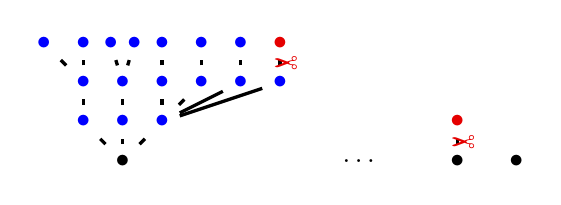
\begin{tikzpicture}[very thick, scale=0.25]
      \node (hn1) at (4,0){$\bullet$};
      \node[blue] (hn2) at (2,2) {$\bullet$};
      \node[blue] (hn3) at (2,4) {$\bullet$};
      \node[blue] (hn4) at (0,6){$\bullet$};
      \node[blue] (hn5) at (2,6){$\bullet$};
      \draw (hn1) -- (hn2) ;
      \draw (hn2) -- (hn3) ;
      \draw (hn3) -- (hn4) ;
      \draw (hn3) -- (hn5) ;
      \node [blue](hn2b) at (4,2) {$\bullet$};
      \node [blue](hn3b) at (4,4) {$\bullet$};
      \node [blue](hn4b) at (3.4,6){$\bullet$};
      \node [blue] (hn5b) at (4.6,6){$\bullet$};
      \draw (hn1) -- (hn2b) ;
      \draw (hn2b) -- (hn3b) ;
      \draw (hn3b) -- (hn4b) ;
      \draw (hn3b) -- (hn5b) ;
      \node [blue](hn2c) at (6,2) {$\bullet$};
      \node [blue](hn3c) at (6,4) {$\bullet$};
      \node [blue](hn4c) at (6,6){$\bullet$};
      \draw (hn1) -- (hn2c) ;
      \draw (hn2c) -- (hn3c) ;
      \draw (hn3c) -- (hn4c) ;
      \node [blue](hn3d) at (8,4) {$\bullet$};
      \draw (hn2c) -- (hn3d) ;
      \node [blue](hn4d) at (8,6) {$\bullet$};
      \draw (hn3d) -- (hn4d) ;
      
      \node [blue](hn3e) at (10,4) {$\bullet$};
      \draw (hn2c) -- (hn3e) ;
      \node [blue](hn4e) at (10,6) {$\bullet$};
      \draw (hn3e) -- (hn4e) ;

      \node [blue](hn3f) at (12,4) {$\bullet$};
      \draw (hn2c) -- (hn3f) ;
      \node [red!90!black](hn4f) at (12,6) {$\bullet$};
      \draw (hn3f) -- node[red!90!black,
      font=\small,sloped,shift={(0.01,-0.075)},
      rotate=90]{\textbf{\ding{34}}} (hn4f) ;

      \node at (16,0) {$\dots$} ;

      \node [black](hn4h) at (21,0) {$\bullet$};
      \node [red!90!black](hn4g) at (21,2) {$\bullet$};
      \draw (hn4h) -- node[red!90!black,
      font=\small,sloped,shift={(0.01,-0.075)},
      rotate=90]{\textbf{\ding{34}}} (hn4g) ;

      
      \node [black](hn4f) at (24,0) {$\bullet$};
      
    \end{tikzpicture}
    \caption{At $t=4,\dots,\textcolor{red}{x}-1,\textcolor{red}{x=?}$
      \label{life2}}
  \end{figure}
\end{frame}

%%%%%%%%%%%%%%%%%%%%%%%%%%%%%%%%%%%%%%%%%%%%

\begin{frame}
  \frametitle{The Ketonen-Solovay machinery\footnote{Rapidly Growing {R}amsey Functions (1981)}}
    \begin{block}{Formalization}

      $$\omega^{\omega^2+1}+1 \rplus{1} \omega^{\omega^2+1}
      \rplus{2} \omega^{\omega^2}\times 3 
      \rplus{3} \omega^{\omega^2}\times 2 +
      \omega ^ {\omega \times 4}, \dots,2,1,0$$

      \vspace{6pt}
      
      $$ \omega^{\omega^2+1}+1 \rplus{1,2,3,4,\dots,x} 0$$
    \end{block}
    
      \begin{block}{Small steps}
        At time $i$, 
           $\alpha \rplus{i} \canonseq{\alpha}{i}$,
        where $\canonseq{\alpha}{\_}$ is the \emph{canonical sequence} of $\alpha$.
        \begin{itemize}
        \item $\canonseq{0}{i}=0$
        \item $\canonseq{\beta+1}{i}=\beta$
         \item If $\lambda$ is a limit ordinal, then $\lambda$ is the $\omega$-limit of $\canonseq{\lambda}{\_}$.
        \end{itemize}
    \end{block}
  
    
      % We associate a hydra to each ordinal \textcolor{mathcolor}{$\alpha<\epsilon_0$} (in Cantor normal form). For instance, the first hydra of our example is the image of \textcolor{mathcolor}{$\omega^{\omega^2+1}+1$}.
    
 
   
 
  \end{frame}

%%%%%%%%%%%%%%%%%%%%%%%%%%%%%%%%%%%%%%%%
\begin{frame}
   
     \begin{block}{}
       \begin{itemize}
       \item In Coq, canonical sequences are defined by structural recursion on ordinal terms in Cantor normal form.
         
   {\color{mathcolor}
         $$\canonseq{\omega^{\omega^{\omega+1}+1}}{42}=
         \omega^{\omega^{\omega+1}}\times 42$$
         }
         
         \input{../../movies/snippets/Canon/canonExamplesb}
       \item Not the same definition as in K. \& S.'s article, but same abstract properties (monotony, limits, \dots).
       \end{itemize}
     \end{block}
\end{frame}

%%%%%%%%%%%%%%%%%%%%%%%%%%%%%%%%%%%%%%
  \begin{frame}
    \frametitle{Paths and accessibility}
    \begin{block}{Theorem (K. \& S., 1981) }
      % If $\beta<\alpha<\epsilon_0$, there exists $i$ and $l$ in $\mathbb{N}$ such that $ \alpha \rplus{i, i+1, i+2, \dots,l} \beta$.

      \vspace{6pt}


          \label{fig:accessibility}
        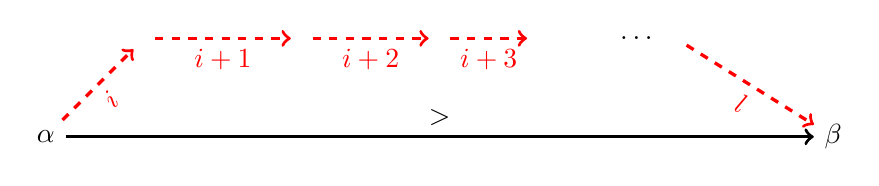
\begin{tikzpicture}[very thick, scale=0.25]
\node (alpha) at (0,0) {$\alpha$};
    \node (beta) at (40, 0){$\beta$};
  

  \draw[->, very thick,black] (alpha)--  node [above]{$>$} (beta);

  \node (alpha1) at (5,5) {};
  \node (alpha2) at (13,5) {};
    \node (alpha3) at (20,5) {};
  \node (alpha4) at (25,5) {};
  \draw [->, dashed,very thick,red] (alpha)-- node [below, rotate=40]{$i$}  (alpha1);
  \draw [->, dashed,very thick,red] (alpha1)-- node [below]{$i+1$}  (alpha2);
   \draw [->, dashed,very thick,red] (alpha2)-- node [below]{$i+2$}  (alpha3);
    \draw [->, dashed,very thick,red] (alpha3)-- node [below]{$i+3$}  (alpha4);
  \node (dots) at (30,5) {$\dots$};
  \node (search) at (32,5){};
 \draw [->, dashed, very thick,red] (search)-- node [below, rotate=-26]{$l$}  (beta);
\end{tikzpicture}

%\pause
\textbf{Remark:} The proof is not trivial. The built path could miss $\beta$!

\vspace{4pt}

\textbf{Cor:} There is no decreasing measure mapping hydras to  $[0, \mu)$ (for any $\mu<\epsilon_0$)  for proving the termination of the considered kind of hydra battles.

\end{block}


    
  \end{frame}


%%%%%%%%%%%%%%%%%%%%%%%%%%%%%%%%%%%%%%%% 
\begin{frame}
  \frametitle{Fast growing hierarchies of arithmetic functions}




\begin{block}{}
 
  {\small
\textbf{Hardy Hierarchy (variant)}
    
 Let us define \textcolor{mathcolor}{$H'_\alpha(i)$} as the least $l$ such that \textcolor{mathcolor}{$\alpha_l=0$} (Figure page.~\pageref{fig:accessibility}). 
 {\color{mathcolor}
\begin{align}
  H'_0(i) & = i\\
  H'_{\beta+1}(i) &=H'_\beta(i+1) \\
  H'_\lambda(i) &= H'_{(\canonseq{\lambda}{i+1})}(i)  \quad\textit{($\lambda$ limit ordinal)} 
\end{align}}
 

\vspace{4pt}

\textbf{Wainer hierarchy (variant)}


We use also the following family in our proofs.

{\color{mathcolor}
\begin{align}
F_0(i)& =i+1\\
F_{\beta+1}(i)&= (F_\beta)^{(i+1)}(i)\\
F_\lambda(i) &= F_{(\canonseq{\lambda}{i})} (i) \quad \textit{($\lambda$ limit ordinal)}
\end{align}}}
\end{block}
\end{frame}

%%%%%%%%%%%%%%%%%%%%%%%%%%%%%%%%%%%%%%%%

%%%%%%%%%%%%%%%%%%%%%%%%%%%%%%%%%%%%%%%%%

% \begin{frame}[fragile]
 
%       \begin{block}{}
%     The functions \textcolor{mathcolor}{$H'_\alpha, F_\alpha\;(\alpha< \epsilon_0)$} are implemented with \textcolor{plugincolor}{coq-equations}.
%     \vspace{5pt}
%     \begin{footnotesize}
%       \inputsnippets{../Hprime_HprimeDef}   
%     \end{footnotesize}

 
%   \end{block}

% \end{frame}


\begin{frame}[fragile]
  \begin{block}{Examples}
         
      {\color{mathcolor}
      
    \begin{align*}
      H'_{\omega^3}(k) \geq\, & \textit{hyper\_exp2}(k+1) \\
      H'_{\omega^\omega}(k)=\,& \textbf{let}\,F\;f\;i := f^{(i+1)}(i)\,
                      \textbf{in}\, F^{(k)}(\lambda k.\,2k+1)\,k\\
    \end{align*}
       }%mathcolor
  \end{block}
  

\begin{block}{Lemmas (after K.\& S.)}
   \begin{itemize} 
    \item \textcolor{mathcolor}{$H'_\alpha$} is strictly monotonous
    
     \item  If $\alpha>0$ then \textcolor{mathcolor}{$ i < H'_\alpha(i)$} for all $i$
    
    \item   $H'_\alpha(i) < H'_{\alpha+1}(i) \; (i \not=0)$
    
       \item     If \textcolor{mathcolor}{$\alpha \rplus{n,n,\dots,n} \beta$} then \textcolor{mathcolor}{$H'_\beta(n)\leq H'_\alpha(n)$} 
         

       \end{itemize}
       (Proof by mutual transfinite induction)
 \end{block}  
  
    
\end{frame}
 

%%%%%%%%%%%%%%%%%%%%%%%%%%%%%%%%%%%%%%%


%%%%%%%%%%%%%%%%%%%%%%%%%%%%%%%%%%%%%%%%%%%%

\begin{frame}
  
  \begin{block}{Theorems}
    \begin{itemize}
    \item $F_\alpha$ is primitive recursive iff $\alpha<\omega$.
     \item  
    The function which computes the length of hydra battles
    for $\alpha$ (according to the initial index) is not primitive recursive
    (for $\alpha\geq \omega^\omega$).

    \end{itemize}
    
    
  
  \begin{block}{Sketch of proof:}

   We apply monotony properties and the famous lemma:
    \vspace{5pt}
    
       \begin{quote}
      {\color{mathcolor}
        For any $n$-ary primitive recursive  function $f$, 
        there exists some $q$ such that the following inequality holds:
         \[\forall\,x_1,\dots,x_n,  
          f(x_1,\dots,\,x_n)\leq\textrm{Ack}(q,\textrm{max}(x_1,\dots,x_n))\]}
    \end{quote}
    (Proof by induction on any primitive recursive function of any arity.)
  \end{block}
  
  \end{block}
\end{frame}

%%%%%%%%%%%%%%%%%%%%%%%%%%%%%%%%%%%%%%%%%%%% 



\begin{frame}
  \frametitle{}
  \begin{scriptsize}
    \inputsnippets{./SchemePrimRecInda}
  \end{scriptsize}
\end{frame}

%%%%%%%%%%%%%%%%%%%%%%%%%%%%%%%%%%%%%%%%%%%



%%%%%%%%%%%%%%%%%%%%%%%%%%%%%%%%%%%%%%%%%%
\section{Project Organization}
% \begin{frame}
%   \frametitle{Project  Organization}
%   \begin{itemize}
%    \item Compatibility with \gaia
%   \item Integration with \community
%   \item Documentation with \alectr
%   \item Package dependencies
%   \item Continuous integration
%   \end{itemize}
% \end{frame}

  %%%%%%%%%%%%%%%%%%%%%%%%%%%%%%%%%%%%%%%%%

%%%%%%%%%%%%%%%%%%%%%%%%%%%%%%%%%%%%%%%%%%

\begin{frame}
  \frametitle{Compatibility with Gaia}
  \begin{block}{From \Hydras to \gaia}
    {\footnotesize
      \inputsnippets{./canonDef}
      \inputsnippets{./gcanonLimitOf}}
  \end{block}
  \begin{block}{}
    We experiment also the other direction (importing \texttt{ssete9} lemmas to \Hydras).
  \end{block}
\end{frame}

\begin{frame}
  \frametitle{Maintenance, CI/CD}
 

  \begin{block}{Reverse Dependencies Compatibility Testing}
    Since we have extracted part of {\color{plugincolor}goedel}, now {\color{plugincolor}goedel} depends on {\color{plugincolor}\Hydras}, and thus we are checking in CI that we do not break it (thanks to the \textcolor{lookcolor}{Coq Nix Toolbox},
    which can generate such CI workflows)
  \end{block}

  \begin{block}{}
    With \Hydras, we hope to demonstrate that projects with complex dependencies are feasible to manage using recent advances in build management and infrastructure.
  \end{block}

\end{frame}

%%%%%%%%%%%%%%%%%%%%%%%%%%%%%%%%%%%%%%%%% 
\section{Presenting proofs with \alectr}
\begin{frame}
  \frametitle{Presenting proofs with \alectr}
  \begin{block}{}
    \begin{itemize}
 \item     The continuously evolving version of the book is continuously deployed from the master branch to the \community website.

     \item
      \coq libraries contain \emph{snippet declarations} which are converted during the compilation of the book into \LaTeX\xspace blocks which are inserted into the book.

    \item The order in which \coq code, goals and answers are presented in the book is determined by the difficulty of the mathematical examples, or the assumed level in \coq of the reader, not by the structure of the libraries.
  
  
    \end{itemize}
  \end{block}
\end{frame}

%%%%%%%%%%%%%%%%%%%%%%%%%%%%%%%%%%%%%%%%% 

\begin{frame}[fragile]
\begin{alltt}
{\color{lightblue}{(* begin snippet Ex42a:: no-out *)}}
Example Ex42: omega + 42 + omega^2 = omega^2. 
{\color{lightblue}{(* end snippet Ex42a *)}}
Proof.
  {\color{lightblue}{(* begin snippet Ex42b *)}}
  assert (HAP:= AP_phi0 2). {\color{lightblue}{(* .no-out *)}}
  elim  HAP; intros _ H0; apply H0; clear H0. 
  {\color{lightblue}{(* end snippet Ex42b *)}}
 \end{alltt}
  
\end{frame}

%%%%%%%%%%%%%%%%%%%%%%%%%%%%%%%%%%%%%%%%%%

\begin{frame}
  \begin{small}
    
     \inputsnippets{../Schutte_Ex42a}   

     By definition of additive principal ordinals, 
    it suffices to prove the inequality $\omega+42< \phi_0(2)$.

    \inputsnippets{../Schutte_Ex42b}
    By Lemma \textit{AP\_plus\_closed}, it suffices to prove  $\omega<\omega^2$ and $42<\omega^2$.
  \end{small}

\end{frame}



%%%%%%%%%%%%%%%%%%%%%%%%%%%%%%%%%%%%%%%%

\begin{frame}
    
  \begin{block}{Remarks}
    \begin{itemize}
    \item We could write the book, because we are also the maintainers of the cited \coq source, and could insert the snippet instructions in the \texttt{.v} files. \textcolor{lookcolor}{But what about commenting interesting code from other people (\emph{e.g.},
        \gaia) ?}
    \item The same  piece of \coq code may be used in several documents, with different styles (book, beamer), and thus
      different filters (hiding or showing subgoals, hypotheses, etc.).
      
    \end{itemize}
  \end{block}

  \begin{block}{To do}
    Define a language for
    \begin{itemize}
    \item Searching sentences in any \coq file,
    \item Applying filters in order to generate as many snippets as needed.
    \end{itemize}
  \end{block}
\end{frame}
%%%%%%%%%%%%%%%%%%%%%%%%%%%%%%%%%%%%%%%%%%

%%%%%%%%%%%%%%%%%%%%%%%%%%%%%%%%%%%%%%% 

\begin{frame}
  \frametitle{Conclusion and perspectives}
  \begin{block}{}
    \begin{itemize}
    \item \Hydras wants to provide  a connection between scientific litterature and proof assistant technology:
      \begin{itemize}
      \item For the mathematician, it gives a concrete view of the mathematical contents: full proofs, examples, computable functions whenever possible, etc.
        \item  For the \coq learner, it provides a consistent set of examples,
allowing to present and compare various formalization and proving techniques.
      \end{itemize}
    \end{itemize}
  \end{block}
  \end{frame}

%%%%%%%%%%%%%%%%%%%%%%%%%%%%%%%%%%%%%%%%%%%%%%

\begin{frame}[fragile]
  \frametitle{Perspectives}
  \begin{block}{Library on ordinals}
      \begin{itemize}
  \item \gaiahydra:
    \begin{itemize}
    \item Remove definition duplicates
     \item types \texttt{T2}, \texttt{T3}, connection between 
    Schütte's model with \texttt{ssete10} (Bourbaki' set theory).
    \end{itemize}
    
  
    \item Formalization by Minki Cho, using a different representation.
{\color{darkorange}
\begin{verbatim}
Inductive Ord.t :=
| Ord.build: 
    forall (A: Type), (A -> Ord.t) -> Ord.t.
\end{verbatim}
}  
    \end{itemize}

  \end{block}
\end{frame}




%%%%%%%%%%%%%%%%%%%%%%%%%%%%%%%%%%%%%%%%%%%

\begin{frame}
  \begin{block}{}
    \begin{itemize}
      \item More results about hyper-complexity and fast growing functions
    \item New toolchain for \alectr
    \item More proof and specification patterns
    \item More examples and exercises
    \item etc.
    \end{itemize}
  \end{block}
\end{frame}

  \begin{frame}
\frametitle{Call to contributors}
  \begin{block}{}
  {\color{plugincolor}\Hydras} and  {\color{plugincolor}\community} are on GitHub. {\color{cyan}Please contribute, reuse!}
      \begin{itemize}
      \item New chapters
      \item Any correction or improvement (text and/or proofs)
        
  
    \end{itemize}
     \end{block}
 
  
\end{frame}


\end{document}

\begin{frame}
  \frametitle{Ordinals in \coq}
  
  \begin{block}{}
    Ordinals less than {\color{mathcolor}$\omega^\omega, \epsilon_0,  \Gamma_0$} are represented as \emph{ordinal notations}: comparison, canonical sequences, partition limit/successors/zero ordinals are implemented by certified functions, allowing the user to write proofs by computation.

    \begin{footnotesize}
      \inputsnippets{./ONDef}

      \inputsnippets{../E0_Ex42}
    \end{footnotesize}

    
    
  \end{block}
\end{frame}
